\section{Beskrivning}
Detta avsnitt ger en övergripande beskrivning av applikationen i sig, dess funktionalitet, dess tilltänkta användare samt begränsningar för applikationens utformning.

\subsection{Beskrivning av applikationen}
Applikationen är ett verktyg för att tydligt få en överblick över händelser och flöden i CI-processer för ett system, exempelvis byggen och tester. Applikationens målgrupp är företag som bedriver mjukvaruutveckling med större utvecklingsteam. Ett företag i målgruppen använder sig i dagsläget av CI och vill kunna upptäcka flaskhalsar och förbättra sitt arbetsflöde. Applikationen är en webbaserad tjänst skriven i JavaScript. Data som visualiseras i applikationen kan komma från valfritt CI-system via ramverket Eiffel. Händelser och flöden visualiseras genom interaktiva grafer där användaren kan välja att visa data i flera olika nivåer för att kunna dra slutsatser sitt utvecklingsflöde. 

\begin{figure}[h]
    \centering
    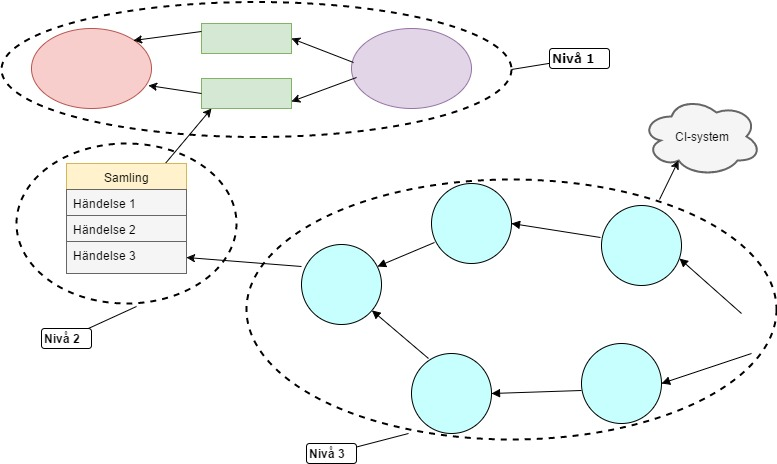
\includegraphics[width=\textwidth]{Visualization}
    \caption{De olika nivåerna av systemet, godtyckligt färgade.}
    \label{fig:system_overview}
\end{figure}
	
\subsection{Funktioner}
Applikationen har en aggregerad och sammanfattad vy av systemet (nivå 1 i figur \ref{fig:system_overview}). Varje nod i grafen på denna nivå representerar varsin typ av händelse, till exempel tester, byggen eller inspektioner. I denna vy slås alla händelser av samma typ samman till en nod. Användaren kan se en detaljerad samling av en viss typ av händelser genom att välja en nod i den aggregerade vyn (nivå 2 i figur \ref{fig:system_overview}). Genom att välja en av händelserna i samlingen kan användaren se ett händelseförlopp för den valda händelsen (nivå 3 i figur \ref{fig:system_overview}). I händelseförloppet kommer händelser som påverkat varandra att vara sammankopplade. 

\newpage

\subsection{Användaregenskaper}
Applikationen riktar sig till användare på alla nivåer inom mjukvaruutveckling, men främst till personer högre upp i hierarkin. Exempel på detta är projektledningen som får en översikt över mjukvaruutvecklingen.
\\ \\
Användaren bör ha god vana vid datorer i allmänhet, kunna navigera i och hantera en webbläsare samt ladda upp och ner filer till och från en hemsida. Användaren bör också vara välbekant med programvaruutveckling, begrepp inom CI, samt den programvara som systemet får sin data från. Användaren ska kunna läsa en README-fil med instruktioner för att installera en programvara. 

\subsection{Begränsningar}
Applikationen kommer köras i en webbläsare, därmed kommer prestandan begränsas av vad webbläsaren klarar av. Internetåtkomst kommer också krävas för att kunna använda applikationen. Renderingen kommer ske med hjälp av JavaScript vilket också kommer sätta ett tak för prestandan.

\subsection{Antaganden och beroenden}
Applikationen förlitar sig på att få Eiffel-data levererad till sig för att kunna utföra visualiseringen och hämtar alltså inte själv in någon data. Den kommer även att implementeras i JavaScript-ramverket Meteor vilket kräver att applikationens användare kan köra en modern JavaScript-applikation i sin webbläsare. Övriga beroenden kan komma att uppstå under projektets gång.